\documentclass{article}
\usepackage[T1]{fontenc}
\usepackage{lmodern}
\usepackage{graphicx}
\usepackage{amsmath,amssymb}
\usepackage[a4paper,margin=2cm]{geometry}
\usepackage[absolute,overlay]{textpos}
\setlength{\TPHorizModule}{1mm}
\setlength{\TPVertModule}{1mm}
\usepackage[indonesian]{babel}
\usepackage{hyperref}
\setlength{\emergencystretch}{2em}
% unit: Halaman 21

\begin{document}

% === Halaman 21 (python/native) ===

21

From left to right: Adi Shamir, Ron Rivest, Len Adleman, Ralph Merkle, Martin 

Hellman, and Whit Diffie (Picture courtesy of Eli Biham, taken at the presentation on 

Monday August 21 at Crypto 2000, an IACR conference

The IEEE Koji Kobayashi Computers and Communications Award

The 1999 award was given to Diffie, Hellman and Merkle for "For the revolutionary invention of public 

key cryptosystems which form the foundation for privacy, integrity and authentication in modern 

communication systems."

The 2000 award was given to Rivest, Shamir and Adleman "For the revolutionary invention of the RSA 

public key cryptosystem which is the first to be widely-adopted."

Sumber: http://www.merkle.com/merkleDir/KobayashiAward.html

Rinaldi M/II4020 Kriptografi

% deskripsi: gambar native xref 106
\noindent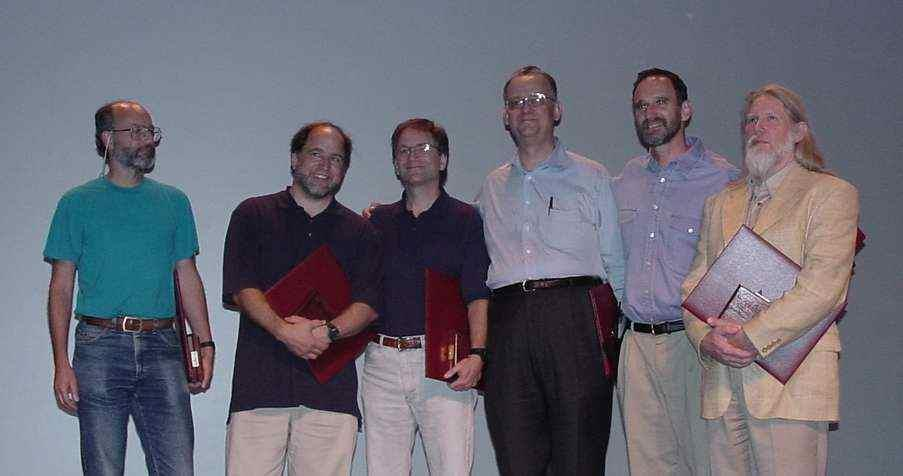
\includegraphics[width=0.85\textwidth]{../../images/python/page_021_img_01.jpeg}

\end{document}
